\newpage
\section{Preliminary Analysis With Synthetic Data}
\label{sec:synthetic-data}
To demonstrate that the \inlabru method is able to correclty identify the underlying age and period effects when we apply the LC-model to mortality data, we compare results produced using \inlabru to results produced using \stan. We define some values for the model components in the LC-model, and use these to sample values for synthetic mortality. We display the synthetic random effects, with their associated hyperparameters together with the estimated random effects as estimated by \inlabru and \stan. 

% v10.3 - predictor
\begin{figure}
    \centering
    \textbf{v10.3: Estimated predictor}
    \begin{subfigure}[b]{.85\linewidth}
        \includegraphics[width=\linewidth]{Master Thesis Code/Scripts/Synthetic data/Output/Figures/v10_3_rw2/eta_x_comparison.pdf}
        \caption{The predictor \etaxt displayed as a function of calendar year, for each age group. }
        \label{fig:eta-v10_3-x}
    \end{subfigure}
    
    \begin{subfigure}[b]{.85\linewidth}
        \includegraphics[width=\linewidth]{Master Thesis Code/Scripts/Synthetic data/Output/Figures/v10_3_rw2/eta_t_comparison.pdf}
        \caption{The predictor \etaxt displayed as a function of age, for each available calendar year. }
        \label{fig:eta-v10_3-t}
    \end{subfigure}
    \caption{The predictor \etaxt estimated by \inlabru and \stan displayed together with the synthetic value for the predictor \etaxt.}
    \label{fig:eta-v10_3}
\end{figure}

% v10.3 - random effects
\begin{figure}
    \centering
    \textbf{v10.3: Estimated random effects}
    \begin{subfigure}[b]{.85\linewidth}
        \includegraphics[width=\linewidth]{Master Thesis Code/Scripts/Synthetic data/Output/Figures/v10_3_rw2/random_effects_comparison.pdf}
        \caption{Estimated random effects.}
        \label{fig:random-effects-v10-3-re}
    \end{subfigure}
    
    \begin{subfigure}[b]{.85\linewidth}
        \includegraphics[width=\linewidth]{Master Thesis Code/Scripts/Synthetic data/Output/Figures/v10_3_rw2/hypers_comparison.pdf}
        \caption{Estimated hyperparameters}
        \label{fig:random-effects-v10-3-hyper}
    \end{subfigure}
    \caption{The age and period effects as estimated by \inlabru and \stan, together with the synthetic random effects. }
    \label{fig:random-effects-v10-3}
\end{figure}

% v10.3 - trace
\begin{figure}
    \centering
    \textbf{Male stomach cancer: Trace plots from \stan}
    \begin{subfigure}[b]{.45\linewidth}
        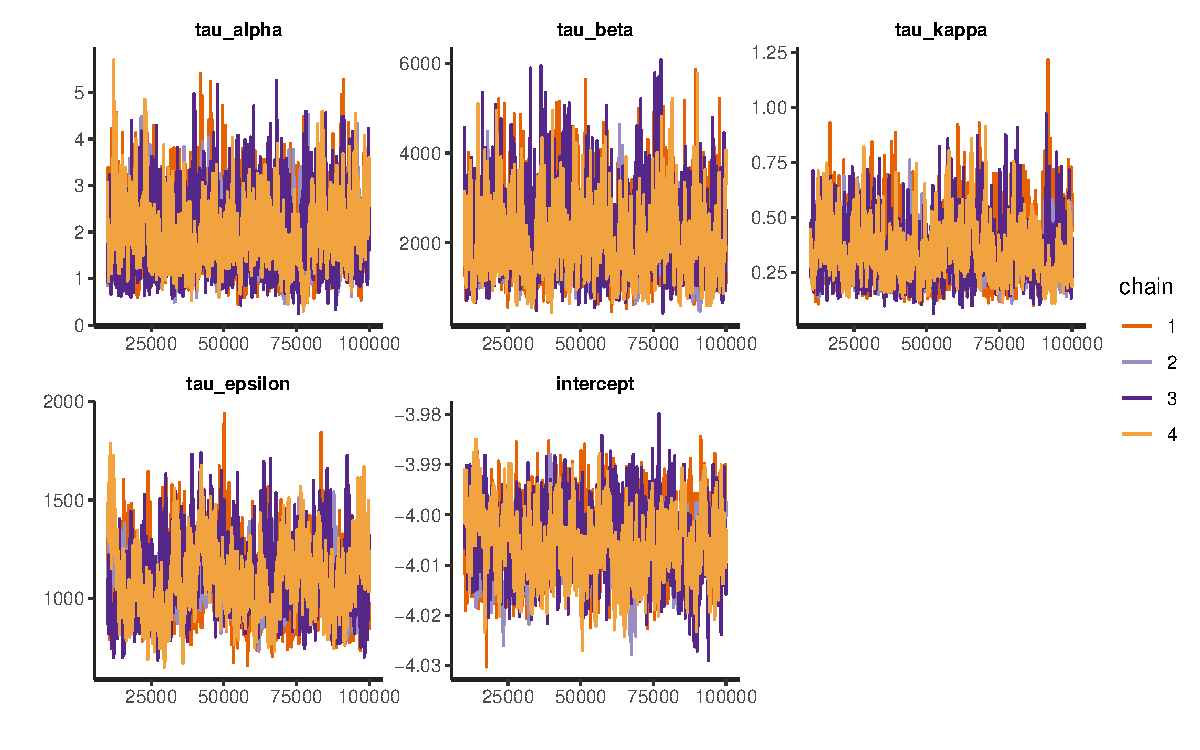
\includegraphics[width=\linewidth]{Master Thesis Code/Scripts/Synthetic data/Stan analyses/v10_3/stan_results/trace_hyperpars.pdf}
        \caption{Trace plots for hyperparameters}
        \label{fig:v10_3-trace-hypers}
    \end{subfigure}
    \begin{subfigure}[b]{.45\linewidth}
        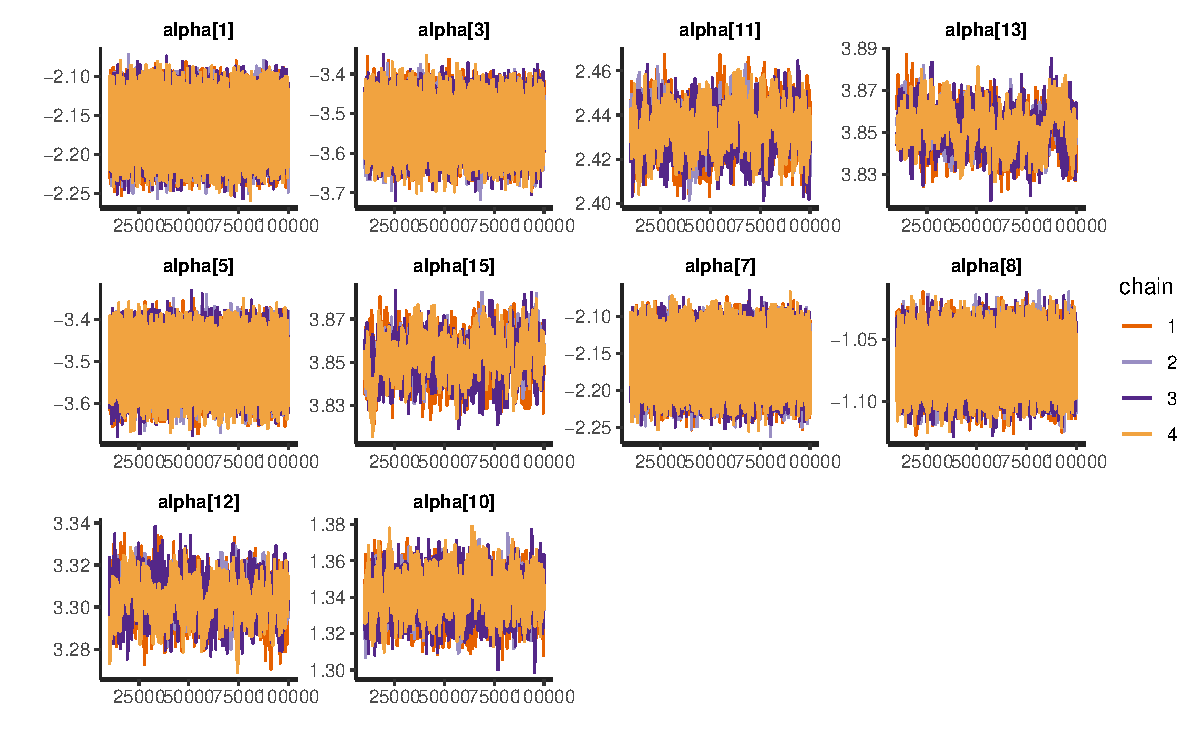
\includegraphics[width=\linewidth]{Master Thesis Code/Scripts/Synthetic data/Stan analyses/v10_3/stan_results/trace_alpha.pdf}
        \caption{Trace plots for selected values of $\alpha_x$}
        \label{fig:v10_3-trace-alpha}
    \end{subfigure}
    
    \begin{subfigure}[b]{.45\linewidth}
        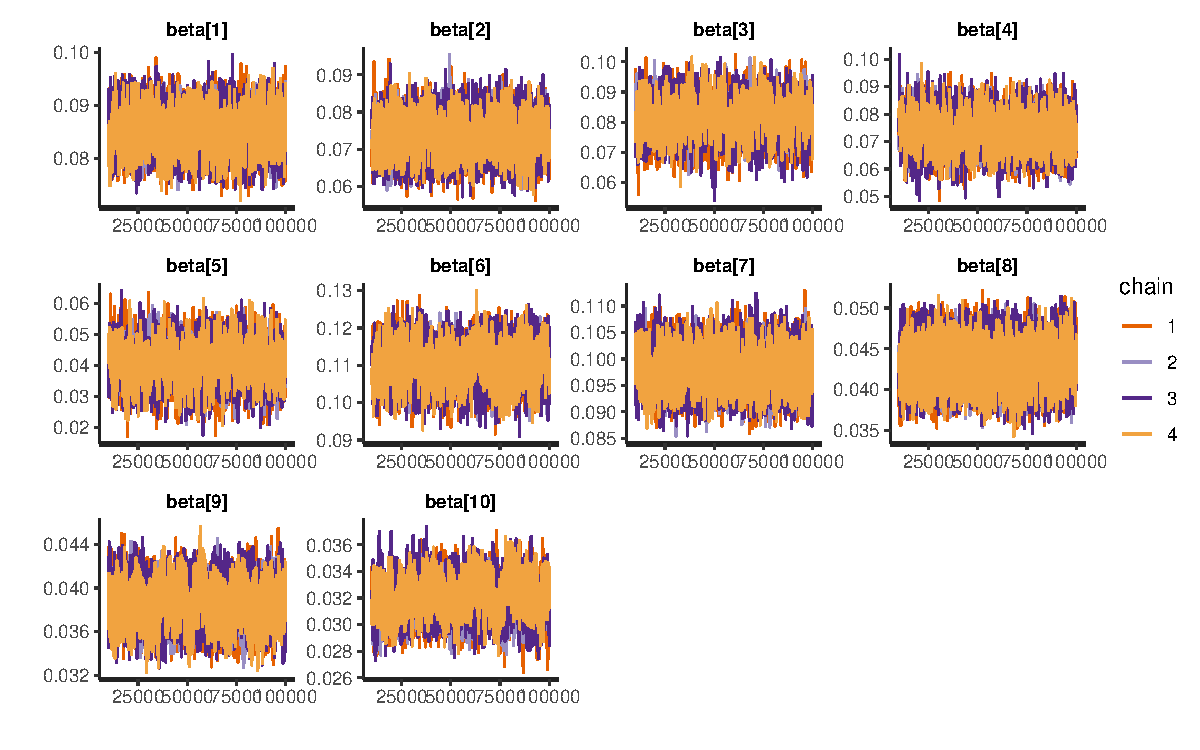
\includegraphics[width=\linewidth]{Master Thesis Code/Scripts/Synthetic data/Stan analyses/v10_3/stan_results/trace_beta.pdf}
        \caption{Trace plots for selected values of $\beta_x$}
        \label{fig:v10_3-trace-beta}
    \end{subfigure}
    \begin{subfigure}[b]{.45\linewidth}
        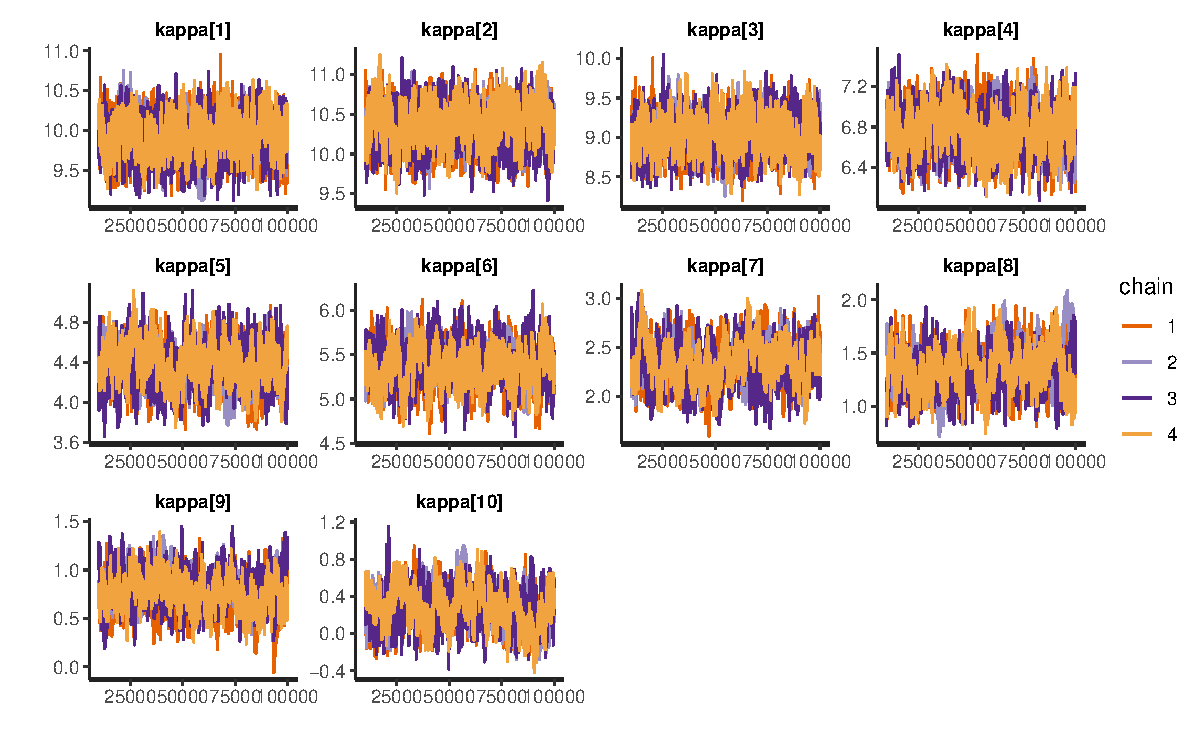
\includegraphics[width=\linewidth]{Master Thesis Code/Scripts/Synthetic data/Stan analyses/v10_3/stan_results/trace_kappa.pdf}
        \caption{Trace plots for selected values of $\kappa_t$}
        \label{fig:v10_3-trace-kappa}
    \end{subfigure}
    \caption{Trace plots from inference using \stan for configuration v10.3. }
    \label{fig:v10_3-trace}
\end{figure}

% v12.3 - predictor
\begin{figure}
    \centering
    \textbf{v12.3: Estimated predictor}
    \begin{subfigure}[b]{.85\linewidth}
        \includegraphics[width=\linewidth]{Master Thesis Code/Scripts/Synthetic data/Output/Figures/v12_3_rw2/eta_x_comparison.pdf}
        \caption{The predictor \etaxt displayed as a function of calendar year, for each age group. }
        \label{fig:eta-v12_3-x}
    \end{subfigure}
    
    \begin{subfigure}[b]{.85\linewidth}
        \includegraphics[width=\linewidth]{Master Thesis Code/Scripts/Synthetic data/Output/Figures/v12_3_rw2/eta_t_comparison.pdf}
        \caption{The predictor \etaxt displayed as a function of age, for each available calendar year. }
        \label{fig:eta-v12_3-t}
    \end{subfigure}
    \caption{The predictor \etaxt estimated by \inlabru and \stan displayed together with the synthetic value for the predictor \etaxt.}
    \label{fig:eta-v12_3}
\end{figure}

% v12.3 - Random effects
\begin{figure}
    \centering
    \textbf{v12.3: Estimated random effects}
    \begin{subfigure}[b]{.85\linewidth}
        \includegraphics[width=\linewidth]{Master Thesis Code/Scripts/Synthetic data/Output/Figures/v12_3_rw2/random_effects_comparison.pdf}
        \caption{Estimated random effects.}
        \label{fig:random-effects-v12-3-re}
    \end{subfigure}
    
    \begin{subfigure}[b]{.85\linewidth}
        \includegraphics[width=\linewidth]{Master Thesis Code/Scripts/Synthetic data/Output/Figures/v12_3_rw2/hypers_comparison.pdf}
        \caption{Estimated hyperparameters}
        \label{fig:random-effects-v12-3-hyper}
    \end{subfigure}
    \caption{The age and period effects as estimated by \inlabru and \stan, together with the synthetic random effects. }
    \label{fig:random-effects-v12-3}
\end{figure}

% v12.3 - trace plots
\begin{figure}
    \centering
    \textbf{Male stomach cancer: Trace plots from \stan}
    \begin{subfigure}[b]{.45\linewidth}
        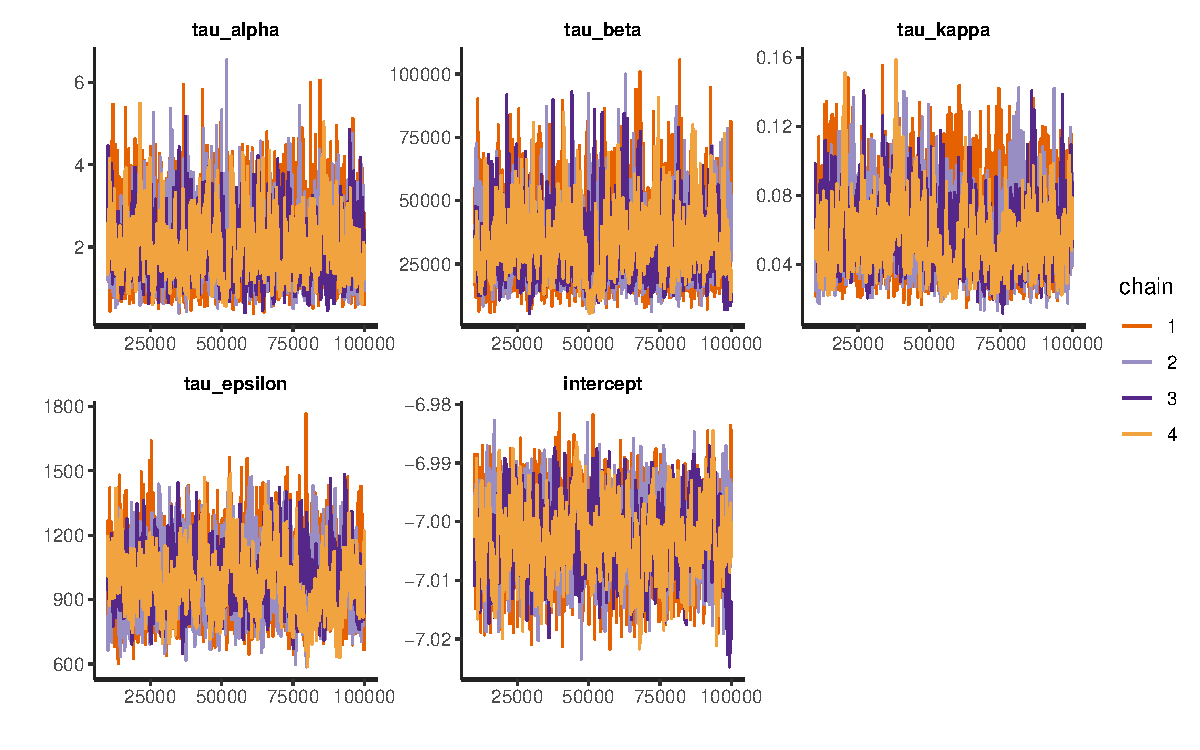
\includegraphics[width=\linewidth]{Master Thesis Code/Scripts/Synthetic data/Stan analyses/v12_3/stan_results/trace_hyperpars.pdf}
        \caption{Trace plots for hyperparameters}
        \label{fig:v12_3-trace-hypers}
    \end{subfigure}
    \begin{subfigure}[b]{.45\linewidth}
        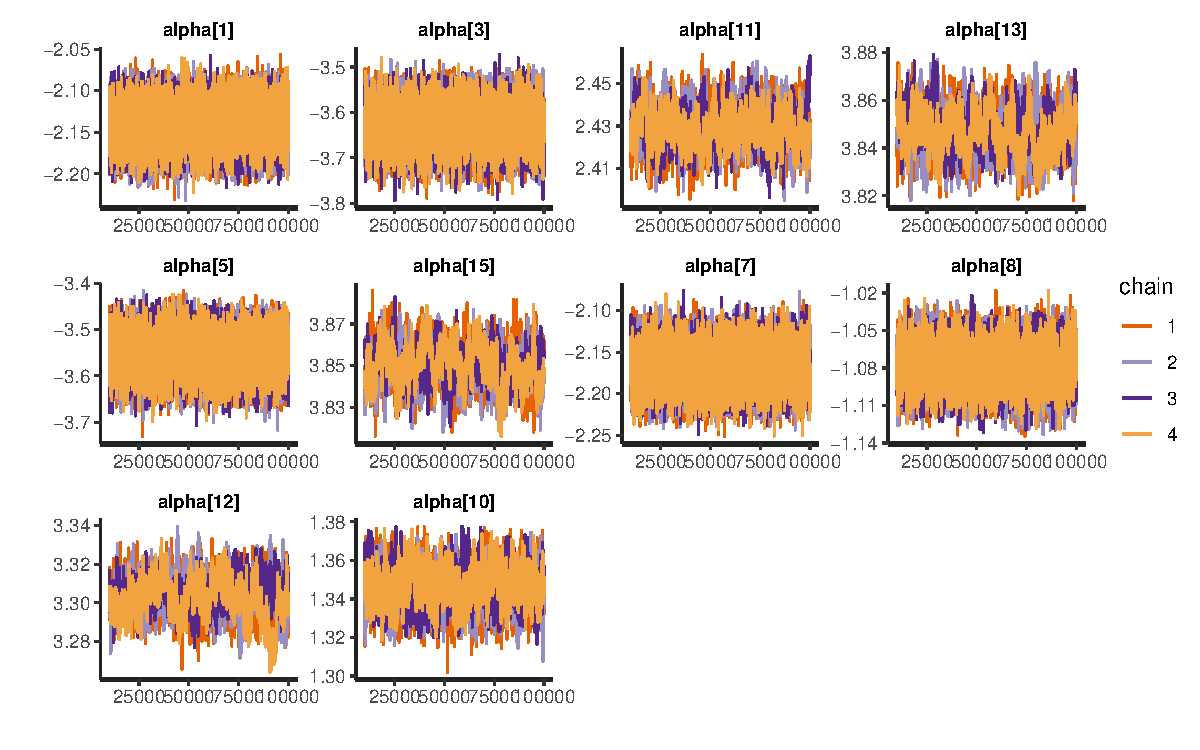
\includegraphics[width=\linewidth]{Master Thesis Code/Scripts/Synthetic data/Stan analyses/v12_3/stan_results/trace_alpha.pdf}
        \caption{Trace plots for selected values of $\alpha_x$}
        \label{fig:v12_3-trace-alpha}
    \end{subfigure}
    
    \begin{subfigure}[b]{.45\linewidth}
        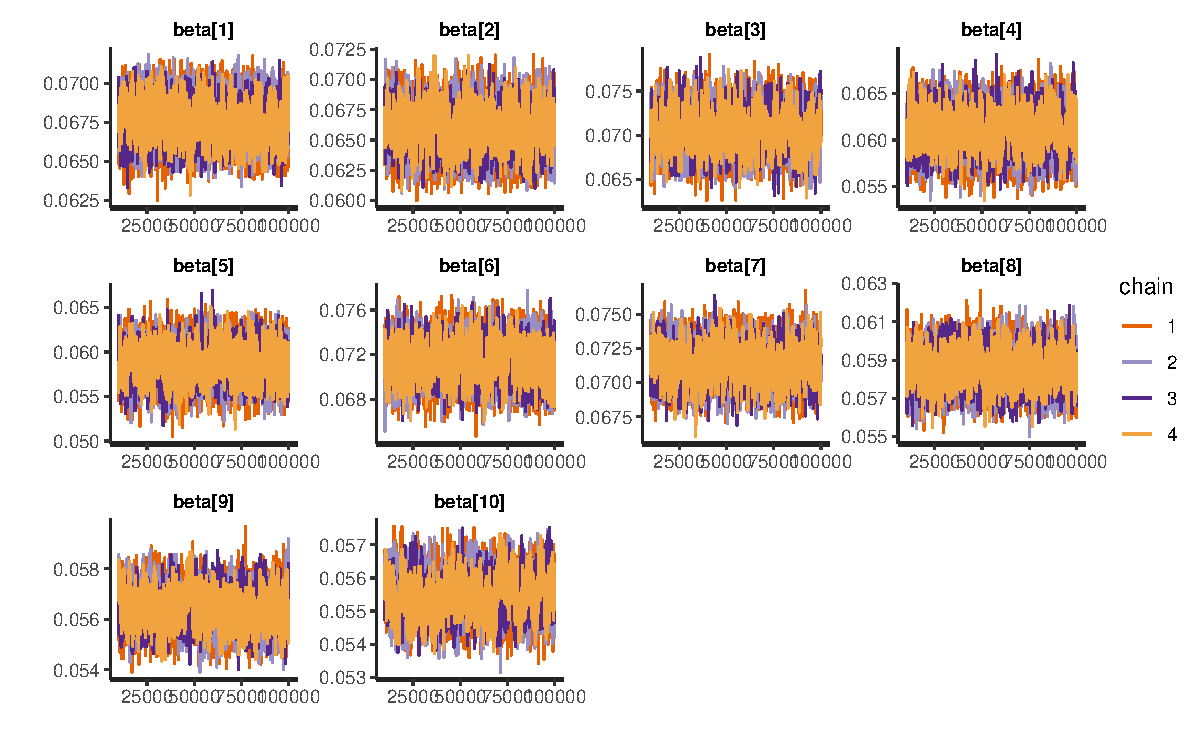
\includegraphics[width=\linewidth]{Master Thesis Code/Scripts/Synthetic data/Stan analyses/v12_3/stan_results/trace_beta.pdf}
        \caption{Trace plots for selected values of $\beta_x$}
        \label{fig:v12_3-trace-beta}
    \end{subfigure}
    \begin{subfigure}[b]{.45\linewidth}
        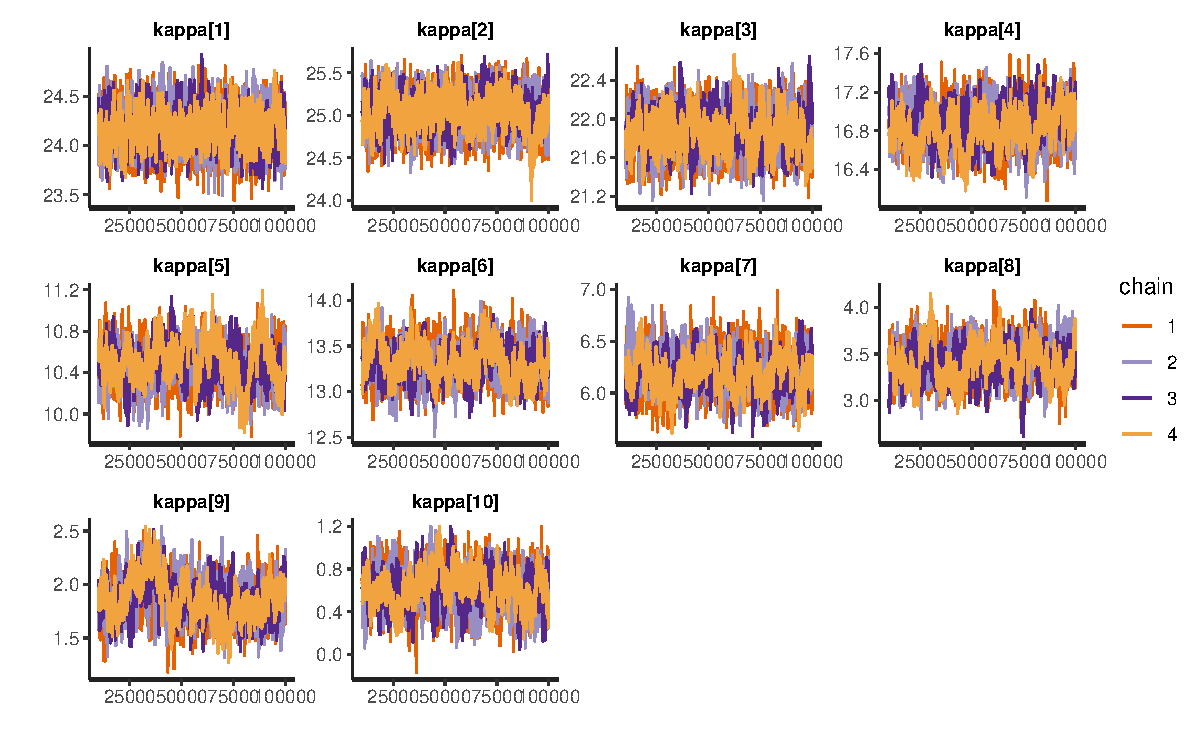
\includegraphics[width=\linewidth]{Master Thesis Code/Scripts/Synthetic data/Stan analyses/v12_3/stan_results/trace_kappa.pdf}
        \caption{Trace plots for selected values of $\kappa_t$}
        \label{fig:v12_3-trace-kappa}
    \end{subfigure}
    \caption{Trace plots from inference using \stan for configuration v12.3. }
    \label{fig:v12_3-trace}
\end{figure}

% Synthetic male stomach - predictor
\begin{figure}
    \centering
    \textbf{Synthetic male stomach: Estimated predictor}
    \begin{subfigure}[b]{.85\linewidth}
        \includegraphics[width=\linewidth]{Master Thesis Code/Scripts/Synthetic data/Output/Figures/synthetic_male_stomach_lc/eta_x_comparison.pdf}
        \caption{The predictor \etaxt displayed as a function of calendar year, for each age group. }
        \label{fig:eta-synthetic_male_stomach_lc-x}
    \end{subfigure}
    
    \begin{subfigure}[b]{.85\linewidth}
        \includegraphics[width=\linewidth]{Master Thesis Code/Scripts/Synthetic data/Output/Figures/synthetic_male_stomach_lc/eta_t_comparison.pdf}
        \caption{The predictor \etaxt displayed as a function of age, for each available calendar year. }
        \label{fig:eta-synthetic_male_stomach_lc-t}
    \end{subfigure}
    \caption{The predictor \etaxt estimated by \inlabru and \stan displayed together with the synthetic value for the predictor \etaxt.}
    \label{fig:eta-synthetic_male_stomach_lc}
\end{figure}

% Synthetic male stomach - random effects 
\begin{figure}
    \centering
    \textbf{Synthetic male stomach: Estimated random effects}
    \begin{subfigure}[b]{.85\linewidth}
        \includegraphics[width=\linewidth]{Master Thesis Code/Scripts/Synthetic data/Output/Figures/synthetic_male_stomach_lc/random_effects_comparison.pdf}
        \caption{Estimated random effects.}
        \label{fig:random-effects-synthetic_male_stomach_lc-re}
    \end{subfigure}
    
    \begin{subfigure}[b]{.85\linewidth}
        \includegraphics[width=\linewidth]{Master Thesis Code/Scripts/Synthetic data/Output/Figures/synthetic_male_stomach_lc/hypers_comparison.pdf}
        \caption{Estimated hyperparameters}
        \label{fig:random-effects-synthetic_male_stomach_lc-hyper}
    \end{subfigure}
    \caption{The age and period effects as estimated by \inlabru and \stan, together with the synthetic random effects. }
    \label{fig:random-effects-synthetic_male_stomach_lc}
\end{figure}

% Synthetic male stomach - trace plots 
\begin{figure}
    \centering
    \textbf{Male stomach cancer: Trace plots from \stan}
    \begin{subfigure}[b]{.45\linewidth}
        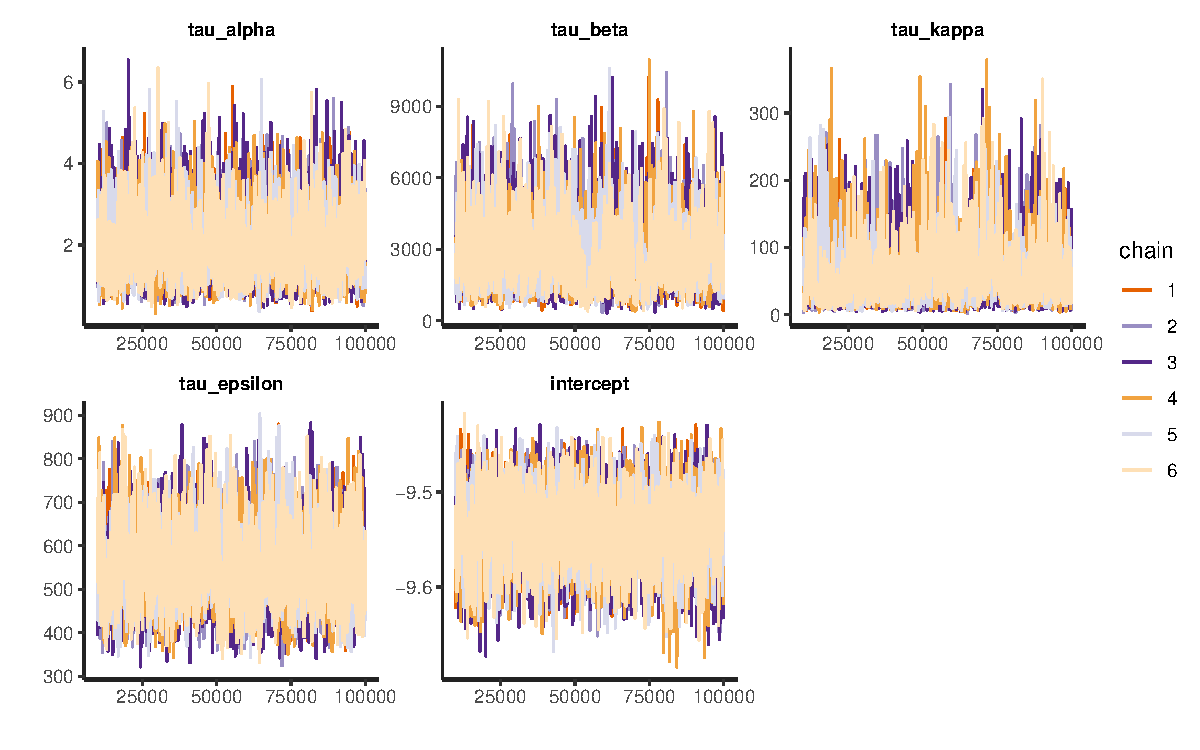
\includegraphics[width=\linewidth]{Master Thesis Code/Scripts/Synthetic data/Stan analyses/synthetic_male_stomach_lc/stan_results/trace_hyperpars.pdf}
        \caption{Trace plots for hyperparameters}
        \label{fig:synthetic_male_stomach_lc-trace-hypers}
    \end{subfigure}
    \begin{subfigure}[b]{.45\linewidth}
        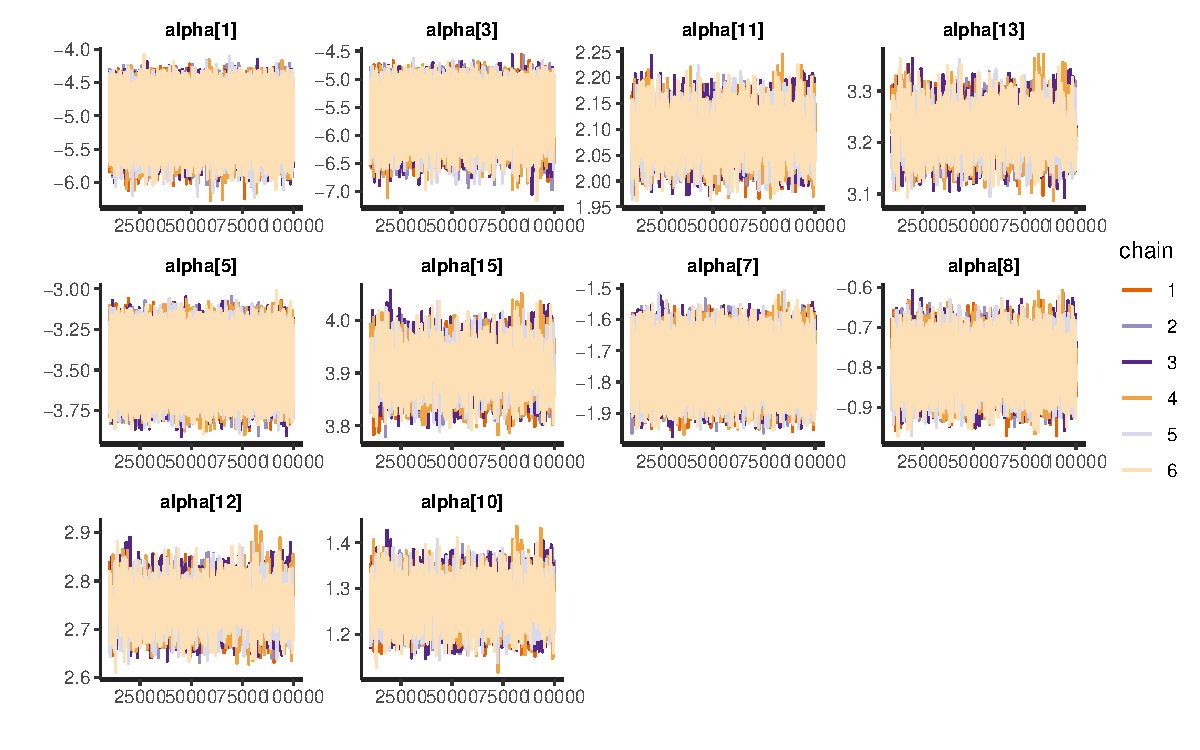
\includegraphics[width=\linewidth]{Master Thesis Code/Scripts/Synthetic data/Stan analyses/synthetic_male_stomach_lc/stan_results/trace_alpha.pdf}
        \caption{Trace plots for selected values of $\alpha_x$}
        \label{fig:synthetic_male_stomach_lc-trace-alpha}
    \end{subfigure}
    
    \begin{subfigure}[b]{.45\linewidth}
        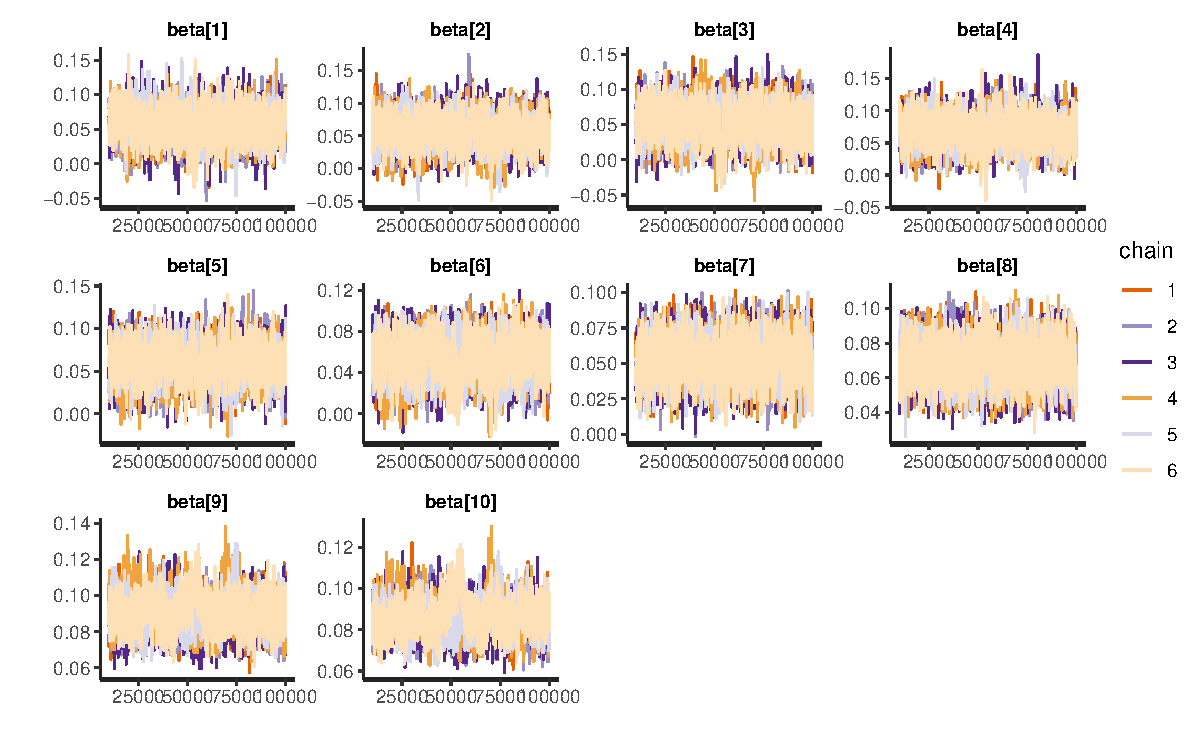
\includegraphics[width=\linewidth]{Master Thesis Code/Scripts/Synthetic data/Stan analyses/synthetic_male_stomach_lc/stan_results/trace_beta.pdf}
        \caption{Trace plots for selected values of $\beta_x$}
        \label{fig:synthetic_male_stomach_lc-trace-beta}
    \end{subfigure}
    \begin{subfigure}[b]{.45\linewidth}
        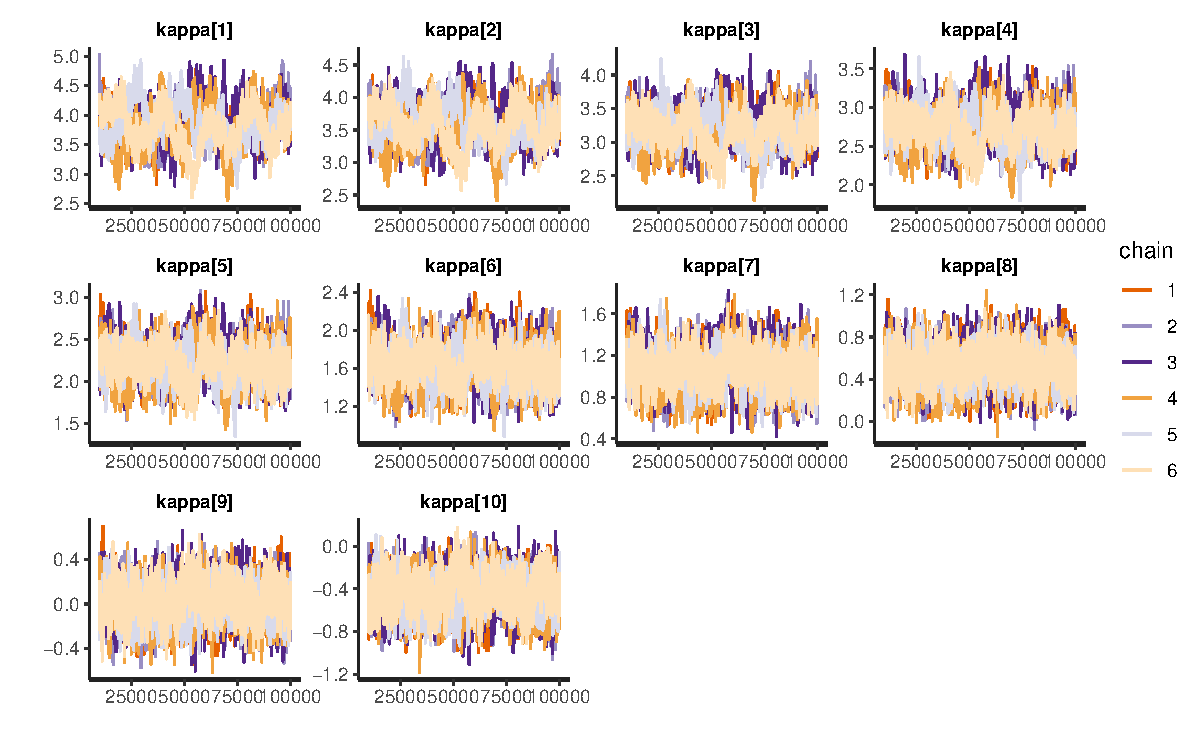
\includegraphics[width=\linewidth]{Master Thesis Code/Scripts/Synthetic data/Stan analyses/synthetic_male_stomach_lc/stan_results/trace_kappa.pdf}
        \caption{Trace plots for selected values of $\kappa_t$}
        \label{fig:synthetic_male_stomach_lc-trace-kappa}
    \end{subfigure}
    \caption{Trace plots from inference using \stan on synthetic male stomach cancer mortality. }
    \label{fig:synthetic_male_stomach_lc-trace}
\end{figure}